%!TEX root = ../main.tex
\chapter{Lavoro ed energia}

\section{Definizione di lavoro di una forza}

La scomposizione delle forze in componenti tangenti e normali fornisce due informazioni ben differenti e diventa interessante quando si studia la dinamica del punto materiale in termini energetici, andando a definire quella grandezza che prende il nome di lavoro.
Si supponga di avere un punto materiale che sta eseguendo uno spostamento in termini infinitesimi pari a $d\vec{r}$ su una traiettoria generica $\Gamma$ soggetto ad una forza $\vec{F}$. In questo contesto si definisce il \textbf{lavoro elementare} della forza $\vec{F}$ compiuto durante lo spostamento vettoriale $d\vec{r}$ la quantità scalare:

\[
	\boxed{d\mathcal{L}=\vec{F}\cdot d\vec{r}}
\]

\begin{figure}[htpb]
	\centering

	\tikzset{every picture/.style={line width=0.75pt}} %set default line width to 0.75pt        

	\begin{tikzpicture}[x=0.75pt,y=0.75pt,yscale=-1,xscale=1]
	%uncomment if require: \path (0,300); %set diagram left start at 0, and has height of 300

	%Curve Lines [id:da4209846702190032] 
	\draw    (107.14,162.09) .. controls (306.54,63.28) and (184.82,253.34) .. (303.5,195.97) .. controls (422.18,138.6) and (463.86,189.98) .. (498.36,170.06) ;
	%Straight Lines [id:da396487998523426] 
	\draw [line width=1.5]    (210,134.4) -- (286.28,78.37) ;
	\draw [shift={(289.5,76)}, rotate = 503.7] [fill={rgb, 255:red, 0; green, 0; blue, 0 }  ][line width=0.08]  [draw opacity=0] (13.4,-6.43) -- (0,0) -- (13.4,6.44) -- (8.9,0) -- cycle    ;
	%Straight Lines [id:da013966627498320783] 
	\draw [line width=1.5]    (210,134.4) -- (242.69,149.11) ;
	\draw [shift={(246.33,150.75)}, rotate = 204.23] [fill={rgb, 255:red, 0; green, 0; blue, 0 }  ][line width=0.08]  [draw opacity=0] (13.4,-6.43) -- (0,0) -- (13.4,6.44) -- (8.9,0) -- cycle    ;
	%Shape: Arc [id:dp12128273572561565] 
	\draw  [draw opacity=0] (226.39,122.26) .. controls (228.91,125.65) and (230.4,129.85) .. (230.4,134.4) .. controls (230.4,137.04) and (229.9,139.56) .. (228.99,141.88) -- (210,134.4) -- cycle ; \draw   (226.39,122.26) .. controls (228.91,125.65) and (230.4,129.85) .. (230.4,134.4) .. controls (230.4,137.04) and (229.9,139.56) .. (228.99,141.88) ;
	%Shape: Boxed Line [id:dp22162093486060597] 
	\draw [line width=0.75]  [dash pattern={on 0.84pt off 2.51pt}]  (289.5,76) -- (254.06,154.75) ;
	%Straight Lines [id:da0719027115068891] 
	\draw [line width=0.75]  [dash pattern={on 0.84pt off 2.51pt}]  (255.22,154.75) -- (210,134.4) ;

	% Text Node
	\draw (295.67,88.4) node    {$\vec{F}$};
	% Text Node
	\draw (211.57,155.9) node    {$d\vec{r}$};
	% Text Node
	\draw (244.87,126) node    {$\vartheta $};
	% Text Node
	\draw (470.67,157.6) node    {$\Gamma $};

	\end{tikzpicture}
\end{figure}
\FloatBarrier
Visto che si parla di uno spostamento infinitesimo, la quantità di lavoro che si ottiene è infinitesima e pertanto la si indica come $d\mathcal{L}$.
Ci si accorge che, andando a risolvere il prodotto scalare, esso vale:

\[
	\norm{\vec{F}}\norm{d\vec{r}}\cos\vartheta
\]

Si possono presentare tre casi:

\begin{itemize}
	\item $\vec{F}$ forma con $d\vec{r}$ un angolo minore di $\frac{\pi}{2}$, per cui l'accelerazione tangente è concorde con la velocità e la fa aumentare: $d\mathcal{L}$ risulta positivo e viene chiamato lavoro \textbf{motore}. Vuol dire che la forza $\vec{F}$ sta fungendo da motore, permette al corpo di proseguire nella sua direzione e aumentare la velocità.
	\item $\vec{F}$ forma un angolo maggiore di $\frac{\pi}{2}$ con $d\vec{r}$, il punto viene frenato e $d\mathcal{L}$ risulta negativo (lavoro \textbf{resistente}). La forza resistente ha l'effetto di rallentare il moto.
	\item Quando la forza è ortogonale allo spostamento si ha che il lavoro è nullo, infatti essa né accelera né rallenta il moto. Capiamo che le forze normali alla traiettoria, le cosiddette \textbf{forze centripete} non compiono mai lavoro.
\end{itemize}

Lungo un arco finito di traiettoria può presentarsi sempre la stessa situazione, così che la velocità finale è maggiore di quella iniziale nel primo caso, minore nel secondo, uguale nel terzo. Tuttavia le varie situazioni possono anche alternarsi e il risultato dipende dalla situazione predominante.
Si noti che $\norm{\vec{F}} \cos\vartheta$ non è altro che la proiezione di $\vec{F}$ in direzione tangente al moto a conferma del fatto che una forza compie lavoro solo se presenta tale componente.

Si è definito il lavoro elementare considerando un tratto molto piccolo di traiettoria. Se la si divide in tanti segmenti infinitesimi, il lavoro totale, complessivo, fatto dalla forza $\vec{F}$ quando il punto materiale si muove sulla traiettoria $\Gamma$ dalla posizione $A$ alla posizione $B$, è la somma di tutti i lavori elementari calcolati su ogni segmento infinitesimo. Essendo una somma continua, si trova un integrale di linea:

\[
	\boxed{\mathcal{L}_{\Gamma, A\to B}=\int_{\Gamma, A\to B} d\mathcal{L}=\int_{\Gamma, A\to B} F_t\,ds}
\]

Il lavoro è dato dalla somma di infinti contributi infinitesimi $F\,ds$.
Facendo l'analisi dimensionale:

\[
	[L]=[F][L]=[M][L]^2[T]^{-2} \to m\,N
\]

Tale unità di misura prende il nome di \emph{Joule}. Una forza di un Newton che agisce in direzione parallela allo spostamento compie il lavoro di un Joule su un metro di spostamento.

\section{Teorema delle forze vive}

Valutare il lavoro fatto da una forza significa valutare l'effetto della forza sulla velocità di un corpo. Questo concetto è esplicitato dal teorema delle forze vive, o dell'energia cinetica. Si consideri una generica porzione della traiettoria di lunghezza $ds$. Immaginiamo che il punto materiale quando si trova in $P$ sia soggetto a $n$ forze.  Applicando il secondo principio della dinamica:

\[
	\vec{F}_1+\vec{F}_2+\dots +\vec{F}_n=m\vec{a}
\]

\begin{figure}[htpb]
	\centering

	\tikzset{every picture/.style={line width=0.75pt}} %set default line width to 0.75pt        

	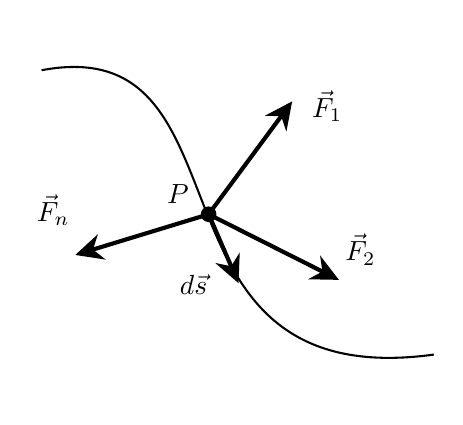
\begin{tikzpicture}[x=0.75pt,y=0.75pt,yscale=-1,xscale=1]
	%uncomment if require: \path (0,300); %set diagram left start at 0, and has height of 300

	%Curve Lines [id:da769583073586938] 
	\draw    (120.5,65) .. controls (226.5,45) and (163.5,222) .. (309.5,202) ;
	%Straight Lines [id:da5627734005611151] 
	\draw [line width=1.5]    (201,134.4) -- (238.87,83.22) ;
	\draw [shift={(241.25,80)}, rotate = 486.5] [fill={rgb, 255:red, 0; green, 0; blue, 0 }  ][line width=0.08]  [draw opacity=0] (13.4,-6.43) -- (0,0) -- (13.4,6.44) -- (8.9,0) -- cycle    ;
	%Shape: Circle [id:dp28223035330479807] 
	\draw  [fill={rgb, 255:red, 0; green, 0; blue, 0 }  ,fill opacity=1 ] (197.75,134.4) .. controls (197.75,132.61) and (199.21,131.15) .. (201,131.15) .. controls (202.79,131.15) and (204.25,132.61) .. (204.25,134.4) .. controls (204.25,136.19) and (202.79,137.65) .. (201,137.65) .. controls (199.21,137.65) and (197.75,136.19) .. (197.75,134.4) -- cycle ;
	%Straight Lines [id:da1868879857416137] 
	\draw [line width=1.5]    (201,134.4) -- (260.18,164.2) ;
	\draw [shift={(263.75,166)}, rotate = 206.73] [fill={rgb, 255:red, 0; green, 0; blue, 0 }  ][line width=0.08]  [draw opacity=0] (13.4,-6.43) -- (0,0) -- (13.4,6.44) -- (8.9,0) -- cycle    ;
	%Straight Lines [id:da1480558067390092] 
	\draw [line width=1.5]    (201,134.4) -- (140.58,152.83) ;
	\draw [shift={(136.75,154)}, rotate = 343.03999999999996] [fill={rgb, 255:red, 0; green, 0; blue, 0 }  ][line width=0.08]  [draw opacity=0] (13.4,-6.43) -- (0,0) -- (13.4,6.44) -- (8.9,0) -- cycle    ;
	%Straight Lines [id:da5486592963361427] 
	\draw [line width=1.5]    (201,134.4) -- (213.81,163.93) ;
	\draw [shift={(215.4,167.6)}, rotate = 246.55] [fill={rgb, 255:red, 0; green, 0; blue, 0 }  ][line width=0.08]  [draw opacity=0] (13.4,-6.43) -- (0,0) -- (13.4,6.44) -- (8.9,0) -- cycle    ;

	% Text Node
	\draw (258.17,82.4) node    {$\vec{F}_{1}$};
	% Text Node
	\draw (274.17,151.4) node    {$\vec{F}_{2}$};
	% Text Node
	\draw (126.17,132.4) node    {$\vec{F}_{n}$};
	% Text Node
	\draw (193.77,168.2) node    {$d\vec{s}$};
	% Text Node
	\draw (186.17,124.6) node    {$P$};

	\end{tikzpicture}
\end{figure}
\FloatBarrier
Se si va a calcolare il lavoro di tutte le forze mentre il punto si starà muovendo sulla traiettoria da $A$ a $B$, andando a sfruttare il secondo principio della dinamica scomposto in componenti tangenti e normali:

\begin{equation*}
	\begin{aligned}
		\mathcal{L} &= \int_{\Gamma, A\to B} F_t\,ds=\int_{\Gamma, A\to B} ma_t\,ds=\int_{\Gamma, A\to B} m\frac{dv}{dt}\,ds= \\
		&= \int_{\Gamma, A\to B} mv\,dv=\frac{1}{2}[ mv^2 ]^B_A=\frac{1}{2}mv^2_B-\frac{1}{2}mv^2_A
	\end{aligned}
\end{equation*}

Questa relazione afferma che quando su un punto materiale agiscono delle forze, il lavoro compiuto da tutte le forze ha l'effetto di variare la velocità del punto materiale in modo tale che $\mathcal{L} = \frac{1}{2}m(v^2_B-v^2_A)$.
Questa espressione rappresenta un'energia a cui si da il nome di energia cinetica. Si definisce l'\textbf{energia cinetica} posseduta da un punto materiale come la quantità energetica:

\[
	\boxed{E_k=\frac{1}{2}mv^2}
\]

Allora il teorema delle forze vive afferma che il lavoro di tutte le forze compiute su un punto materiale provoca la variazione dell'energia cinetica di esso quando si sposta dalla posizione iniziale in $A$ e quella finale in $B$. 

\begin{figure}[htpb]
	\centering

	\tikzset{every picture/.style={line width=0.75pt}} %set default line width to 0.75pt        

	\begin{tikzpicture}[x=0.75pt,y=0.75pt,yscale=-1,xscale=1]
	%uncomment if require: \path (0,300); %set diagram left start at 0, and has height of 300

	%Curve Lines [id:da22223273061886006] 
	\draw    (140.5,85) .. controls (255.33,43) and (248,167) .. (388.67,135) ;
	%Shape: Circle [id:dp7960730507131906] 
	\draw  [fill={rgb, 255:red, 0; green, 0; blue, 0 }  ,fill opacity=1 ] (210.42,81.4) .. controls (210.42,79.61) and (211.87,78.15) .. (213.67,78.15) .. controls (215.46,78.15) and (216.92,79.61) .. (216.92,81.4) .. controls (216.92,83.19) and (215.46,84.65) .. (213.67,84.65) .. controls (211.87,84.65) and (210.42,83.19) .. (210.42,81.4) -- cycle ;
	%Shape: Circle [id:dp1184180970622013] 
	\draw  [fill={rgb, 255:red, 0; green, 0; blue, 0 }  ,fill opacity=1 ] (321.75,138.73) .. controls (321.75,136.94) and (323.21,135.48) .. (325,135.48) .. controls (326.79,135.48) and (328.25,136.94) .. (328.25,138.73) .. controls (328.25,140.53) and (326.79,141.98) .. (325,141.98) .. controls (323.21,141.98) and (321.75,140.53) .. (321.75,138.73) -- cycle ;

	% Text Node
	\draw (228.17,69.73) node    {$A$};
	% Text Node
	\draw (327.5,120.4) node    {$B$};

	\end{tikzpicture}
\end{figure}
\FloatBarrier
Si chiama anche teorema delle forze vive perché comunica che le uniche forze che hanno l'effetto di far variare il valore della velocità sono quelle tangenti al moto.
In realtà la definizione di $E_k$ non è univoca ma è definita a meno di una costante aggiuntiva, che si sceglie uguale a zero in modo tale che un corpo a riposo abbia energia cinetica nulla. In questo modo tale concetto assume anche un significato fisico. La nozione di lavoro infatti, e quindi anche quella di variazione di energia cinetica, è necessariamente legata a quella di spostamento: se non c'è spostamento non può esserci lavoro, qualunque sia la forza applicata. Il lavoro fatto da una forza dipende in generale dalla traiettoria su cui si sta muovendo il corpo. Non si perde la dipendenza dalla traiettoria nella definizione di energia cinetica, infatti, a seconda di essa, il valore con cui il punto arriva in $B$ sarà in generale diverso.

Le due seguenti relazioni:

\[
	\boxed{F_t=ma_t \iff \mathcal{L}_\Gamma=\Delta E_k}
\]

portano ovviamente allo stesso risultato e il loro campo di validità è lo stesso (i sistemi di riferimento inerziali). Si dice che il teorema dell'energia cinetica è invariante rispetto a tali sistemi.

Si può riscrivere il teorema dell'energia cinetica (e anche di conservazione dell'energia meccanica di conseguenza) per i sistemi non inerziali. Si dovrà tenere conto del lavoro compiuto anche da tutte le forze apparenti:

\[
	\mathcal{L}_{\text{F}_{\text{reali}}}+\mathcal{L}_{\text{F}_{\text{app}}}=\Delta E_{k, \text{ rel}}
\]

Nel calcolo del lavoro bisogna valutare quello delle forze mentre il punto materiale si muove sulla traiettoria percepita dall'osservatore relativo. Se le forze apparenti non fossero costanti mentre il punto si muove si tratterebbe di risolvere un'equazione differenziale, problema non che non verrà affrontato.

\section{Forze conservative e non}

\subsection{Esempi di lavoro}

Si espongono in seguito alcuni esempi di calcolo di lavoro compiuto da alcune forze.

\subsubsection{Lavoro della forza peso}

Un punto materiale si sta muovendo da una posizione $A$ a una posizione $B$ sulla traiettoria. Si definisce un asse $z$ rivolto verso l'alto e si chiamano $z_a$ la quota iniziale a cui si trova il punto e $z_b$ quella finale. In un punto generico si va a mettere in evidenza la direzione della forza peso e la direzione dello spostamento. Il lavoro della forza peso lungo la traiettoria $\Gamma$ che va da $A$ a $B$ non è altro che:

\[
	\mathcal{L}_{\Gamma, A \to B}=\int_{\Gamma, A \to B} m\vec{g} \cdot \vec{dr}
\]

In questo caso lo spostamento continua a cambiare la propria direzione mentre la forza peso la mantiene costante. Quindi conviene scomporre $d\vec{r}$ e considerare la sua proiezione su $z$.

\[
	d\vec{r}=dx\vec{u}_x+dy\vec{u}_y+dz\vec{u}_z \quad m\vec{g}=-mg\vec{u}_z
\]

Sopravvive solo la terza componente perché le altre due sono ortogonali alla forza peso.

\[
	\boxed{\mathcal{L}_{\Gamma, A \to B}=\int_{\Gamma, A \to B} -mg\,dz=mg(z_a-z_b)}
\]

\begin{figure}[htpb]
	\centering

	\tikzset{every picture/.style={line width=0.75pt}} %set default line width to 0.75pt        

	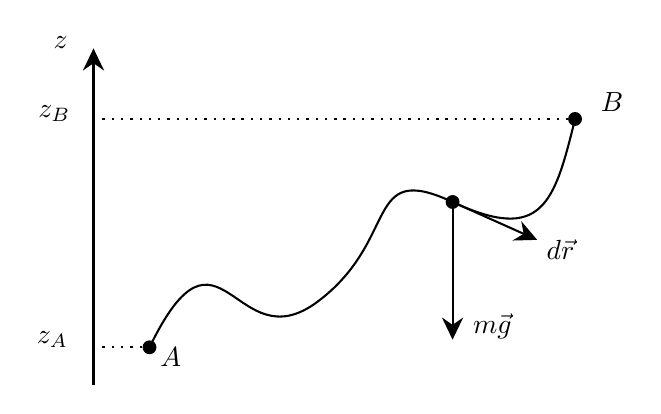
\begin{tikzpicture}[x=0.75pt,y=0.75pt,yscale=-1,xscale=1]
	%uncomment if require: \path (0,300); %set diagram left start at 0, and has height of 300

	%Straight Lines [id:da4567550117967014] 
	\draw    (179.5,226) -- (179.5,67) ;
	\draw [shift={(179.5,64)}, rotate = 450] [fill={rgb, 255:red, 0; green, 0; blue, 0 }  ][line width=0.08]  [draw opacity=0] (10.72,-5.15) -- (0,0) -- (10.72,5.15) -- (7.12,0) -- cycle    ;
	%Straight Lines [id:da8799949196323655] 
	\draw  [dash pattern={on 0.84pt off 2.51pt}]  (179.33,208) -- (206.5,208) ;
	%Curve Lines [id:da992092583362937] 
	\draw    (206.5,208) .. controls (240.5,138) and (247.5,216) .. (287.5,186) .. controls (327.5,156) and (309.5,118) .. (352.5,138) .. controls (395.5,158) and (401.5,139) .. (411.5,98) ;
	%Shape: Circle [id:dp1915008511555767] 
	\draw  [fill={rgb, 255:red, 0; green, 0; blue, 0 }  ,fill opacity=1 ] (203.67,208) .. controls (203.67,206.44) and (204.94,205.17) .. (206.5,205.17) .. controls (208.06,205.17) and (209.33,206.44) .. (209.33,208) .. controls (209.33,209.56) and (208.06,210.83) .. (206.5,210.83) .. controls (204.94,210.83) and (203.67,209.56) .. (203.67,208) -- cycle ;
	%Shape: Circle [id:dp5508839626190245] 
	\draw  [fill={rgb, 255:red, 0; green, 0; blue, 0 }  ,fill opacity=1 ] (408.67,98) .. controls (408.67,96.44) and (409.94,95.17) .. (411.5,95.17) .. controls (413.06,95.17) and (414.33,96.44) .. (414.33,98) .. controls (414.33,99.56) and (413.06,100.83) .. (411.5,100.83) .. controls (409.94,100.83) and (408.67,99.56) .. (408.67,98) -- cycle ;
	%Straight Lines [id:da7581801323720281] 
	\draw  [dash pattern={on 0.84pt off 2.51pt}]  (179.33,98) -- (411.5,98) ;
	%Straight Lines [id:da7547784460352234] 
	\draw    (352.5,138) -- (352.5,201.33) ;
	\draw [shift={(352.5,204.33)}, rotate = 270] [fill={rgb, 255:red, 0; green, 0; blue, 0 }  ][line width=0.08]  [draw opacity=0] (10.72,-5.15) -- (0,0) -- (10.72,5.15) -- (7.12,0) -- cycle    ;
	%Straight Lines [id:da3231983593688519] 
	\draw    (352.5,138) -- (390.51,155.02) ;
	\draw [shift={(393.25,156.25)}, rotate = 204.13] [fill={rgb, 255:red, 0; green, 0; blue, 0 }  ][line width=0.08]  [draw opacity=0] (10.72,-5.15) -- (0,0) -- (10.72,5.15) -- (7.12,0) -- cycle    ;
	%Shape: Circle [id:dp43575236520295135] 
	\draw  [fill={rgb, 255:red, 0; green, 0; blue, 0 }  ,fill opacity=1 ] (349.67,138) .. controls (349.67,136.44) and (350.94,135.17) .. (352.5,135.17) .. controls (354.06,135.17) and (355.33,136.44) .. (355.33,138) .. controls (355.33,139.56) and (354.06,140.83) .. (352.5,140.83) .. controls (350.94,140.83) and (349.67,139.56) .. (349.67,138) -- cycle ;

	% Text Node
	\draw (163.67,61.33) node    {$z$};
	% Text Node
	\draw (160.67,95.33) node    {$z_{B}$};
	% Text Node
	\draw (159.67,204.33) node    {$z_{A}$};
	% Text Node
	\draw (216.67,212.67) node    {$A$};
	% Text Node
	\draw (429.33,89.67) node    {$B$};
	% Text Node
	\draw (371.67,198) node    {$m\vec{g}$};
	% Text Node
	\draw (404.5,161) node    {$d\vec{r}$};

	\end{tikzpicture}
\end{figure}
\FloatBarrier
Si noti che il lavoro non dipende dalla traiettoria ma solo dalla quota finale e da quella iniziale. Questo significa che se il punto per andare da $A$ a $B$ ci va seguendo diverse traiettorie, il lavoro fatto dalla forza peso è lo stesso. Il segno meno significa che quando il punto materiale viene sollevato di quota il lavoro è negativo. Viceversa se è il punto materiale che scivola giù, il lavoro diventa positivo. Infatti, se il punto $B$ si trova in una posizione più bassa di $A$, $AB$ è lo spostamento naturale di un punto $P$ sottoposto alla sola forza peso. Se invece il punto $B$ è più in alto rispetto ad $A$ significa che il punto deve avere una sufficiente velocità iniziale così che la diminuzione di energia cinetica eguagli il lavoro. Altrimenti è necessario applicare al punto un'altra forza il cui lavoro motore superi in modulo il lavoro resistente della forza peso.

\subsubsection{Lavoro di una forza elastica}

Si immagini di avere un punto materiale di massa $M$ vincolato a una molla di costante elastica $k$. La molla viene allungata, per cui il punto materiale oscilla seguendo una legge di moto armonico (che verrà in seguito affrontato). Si è interessati a capire qual è il lavoro fatto dalla forza elastica quando la molla passa per le posizioni generiche $A$ e $B$. Quando allungata, essa genera una forza di richiamo che tende a riportare il punto materiale nella posizione $O$.

\[
	\boxed{\mathcal{L}_{\Gamma, A \to B}=\int_{\Gamma, A \to B} \vec{F}\cdot d\vec{r}= \int_{x_A}^{x_B} -kx\,dx=\frac{1}{2}k(x_A^2-x_B^2)}
\]

\begin{figure}[htpb]
	\centering

	\tikzset{every picture/.style={line width=0.75pt}} %set default line width to 0.75pt        

	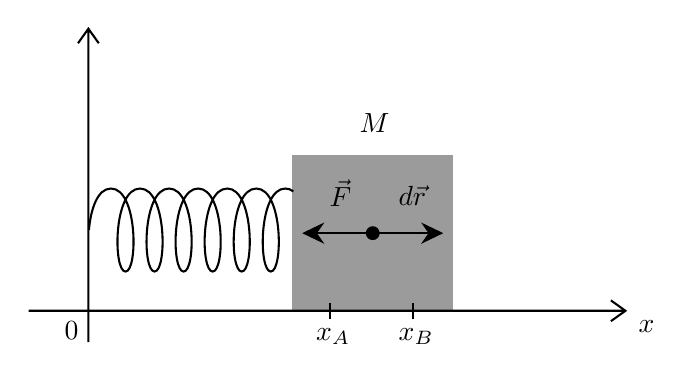
\begin{tikzpicture}[x=0.75pt,y=0.75pt,yscale=-1,xscale=1]
	%uncomment if require: \path (0,300); %set diagram left start at 0, and has height of 300

	%Shape: Rectangle [id:dp4234502411788541] 
	\draw  [draw opacity=0][fill={rgb, 255:red, 155; green, 155; blue, 155 }  ,fill opacity=1 ] (204,129) -- (281.5,129) -- (281.5,204) -- (204,204) -- cycle ;
	%Shape: Axis 2D [id:dp8158083942748016] 
	\draw  (77,203.9) -- (364.5,203.9)(105.75,68) -- (105.75,219) (357.5,198.9) -- (364.5,203.9) -- (357.5,208.9) (100.75,75) -- (105.75,68) -- (110.75,75)  ;
	%Shape: Spring [id:dp9074821559743382] 
	\draw   (106,165) .. controls (106.88,155) and (110.13,145) .. (116.63,145) .. controls (129.63,145) and (129.63,185) .. (123.63,185) .. controls (117.63,185) and (117.63,145) .. (130.63,145) .. controls (143.63,145) and (143.63,185) .. (137.63,185) .. controls (131.63,185) and (131.63,145) .. (144.63,145) .. controls (157.63,145) and (157.63,185) .. (151.63,185) .. controls (145.63,185) and (145.63,145) .. (158.63,145) .. controls (171.63,145) and (171.63,185) .. (165.63,185) .. controls (159.63,185) and (159.63,145) .. (172.63,145) .. controls (185.63,145) and (185.63,185) .. (179.63,185) .. controls (173.63,185) and (173.63,145) .. (186.63,145) .. controls (199.63,145) and (199.63,185) .. (193.63,185) .. controls (187.63,185) and (187.63,145) .. (200.63,145) .. controls (202.08,145) and (203.36,145.5) .. (204.5,146.38) ;
	%Straight Lines [id:da4992112063762819] 
	\draw    (242.75,166.5) -- (273.75,166.5) ;
	\draw [shift={(276.75,166.5)}, rotate = 180] [fill={rgb, 255:red, 0; green, 0; blue, 0 }  ][line width=0.08]  [draw opacity=0] (10.72,-5.15) -- (0,0) -- (10.72,5.15) -- (7.12,0) -- cycle    ;
	%Straight Lines [id:da1169902927225368] 
	\draw    (211.75,166.5) -- (242.75,166.5) ;
	\draw [shift={(208.75,166.5)}, rotate = 0] [fill={rgb, 255:red, 0; green, 0; blue, 0 }  ][line width=0.08]  [draw opacity=0] (10.72,-5.15) -- (0,0) -- (10.72,5.15) -- (7.12,0) -- cycle    ;
	%Shape: Circle [id:dp39681623393842536] 
	\draw  [fill={rgb, 255:red, 0; green, 0; blue, 0 }  ,fill opacity=1 ] (239.92,166.5) .. controls (239.92,164.94) and (241.19,163.67) .. (242.75,163.67) .. controls (244.31,163.67) and (245.58,164.94) .. (245.58,166.5) .. controls (245.58,168.06) and (244.31,169.33) .. (242.75,169.33) .. controls (241.19,169.33) and (239.92,168.06) .. (239.92,166.5) -- cycle ;
	%Straight Lines [id:da5686270262356254] 
	\draw    (222,200.33) -- (222,208) ;
	%Straight Lines [id:da28261884806148196] 
	\draw    (262,200.33) -- (262,208) ;

	% Text Node
	\draw (374.67,211.33) node    {$x$};
	% Text Node
	\draw (243.67,113.33) node    {$M$};
	% Text Node
	\draw (261.83,148.33) node    {$d\vec{r}$};
	% Text Node
	\draw (223.67,216.33) node    {$x_{A}$};
	% Text Node
	\draw (263.67,216.33) node    {$x_{B}$};
	% Text Node
	\draw (97.67,213.33) node    {$0$};
	% Text Node
	\draw (227.17,147.33) node    {$\vec{F}$};

	\end{tikzpicture}
\end{figure}
\FloatBarrier
Anche per la forza elastica è possibile non considerare più la dipendenza dalla traiettoria. Il lavoro fatto dalla molla è lo stesso quando la massa va da $A$ a $B$ oppure quando partendo da $A$ fa un oscillazione completa
e poi torna su $B$. Le reazioni vincolari non vanno considerare perché sono ortogonali allo spostamento.

\subsubsection{Lavoro della forza di attrito radente}

La forza di attrito radente statico non compie lavoro perché, come già ribadito, quando non si ha spostamento non è mai possibile avere lavoro. Si consideri allora la forza di attrito radente dinamico. Sia un corpo appoggiato a un piano scabro con coefficiente di attrito $\mu_d$ che si sta muovendo in avanti. La forza di attrito dinamico sarà tangente al piano di appoggio e opposta allo spostamento.

\[
	\mathcal{L}_{\Gamma, A \to B}=\int_A^B \vec{F}_{\text{attr}} \cdot d\vec{r}
\]

Scomponendo le forze in componenti intrinseche alla traiettoria:

\[
	\vec{F}_{\text{attr}}=-\mu_d\norm{\vec{R}_n} \vec{u}_t \quad d\vec{r}=ds\vec{u}_t
\]

Supponendo che il punto si muova sullo stesso piano, $R_n$ è costante.

\[
	\boxed{\mathcal{L}_{\Gamma, A \to B}=\int_A^B -\mu_d\norm{\vec{R}_n} \,ds=-\mu_d\norm{\vec{R}_n}L_\Gamma}
\]

\begin{figure}[htpb]
	\centering

	% Pattern Info
	 
	\tikzset{
	pattern size/.store in=\mcSize, 
	pattern size = 5pt,
	pattern thickness/.store in=\mcThickness, 
	pattern thickness = 0.3pt,
	pattern radius/.store in=\mcRadius, 
	pattern radius = 1pt}
	\makeatletter
	\pgfutil@ifundefined{pgf@pattern@name@_c6kb6rdxs}{
	\pgfdeclarepatternformonly[\mcThickness,\mcSize]{_c6kb6rdxs}
	{\pgfqpoint{0pt}{-\mcThickness}}
	{\pgfpoint{\mcSize}{\mcSize}}
	{\pgfpoint{\mcSize}{\mcSize}}
	{
	\pgfsetcolor{\tikz@pattern@color}
	\pgfsetlinewidth{\mcThickness}
	\pgfpathmoveto{\pgfqpoint{0pt}{\mcSize}}
	\pgfpathlineto{\pgfpoint{\mcSize+\mcThickness}{-\mcThickness}}
	\pgfusepath{stroke}
	}}
	\makeatother
	\tikzset{every picture/.style={line width=0.75pt}} %set default line width to 0.75pt        

	\begin{tikzpicture}[x=0.75pt,y=0.75pt,yscale=-1,xscale=1]
	%uncomment if require: \path (0,300); %set diagram left start at 0, and has height of 300

	%Shape: Rectangle [id:dp5747589760441774] 
	\draw  [draw opacity=0][pattern=_c6kb6rdxs,pattern size=6.5249999999999995pt,pattern thickness=0.75pt,pattern radius=0pt, pattern color={rgb, 255:red, 155; green, 155; blue, 155}] (115.5,204) -- (396.5,204) -- (396.5,231) -- (115.5,231) -- cycle ;
	%Shape: Rectangle [id:dp5186133906953796] 
	\draw  [draw opacity=0][fill={rgb, 255:red, 155; green, 155; blue, 155 }  ,fill opacity=1 ] (164,129) -- (241.5,129) -- (241.5,204) -- (164,204) -- cycle ;
	%Straight Lines [id:da980881591168157] 
	\draw    (202.75,166.5) -- (295,166.5) ;
	\draw [shift={(298,166.5)}, rotate = 180] [fill={rgb, 255:red, 0; green, 0; blue, 0 }  ][line width=0.08]  [draw opacity=0] (10.72,-5.15) -- (0,0) -- (10.72,5.15) -- (7.12,0) -- cycle    ;
	%Shape: Circle [id:dp803196961729584] 
	\draw  [fill={rgb, 255:red, 0; green, 0; blue, 0 }  ,fill opacity=1 ] (199.92,166.5) .. controls (199.92,164.94) and (201.19,163.67) .. (202.75,163.67) .. controls (204.31,163.67) and (205.58,164.94) .. (205.58,166.5) .. controls (205.58,168.06) and (204.31,169.33) .. (202.75,169.33) .. controls (201.19,169.33) and (199.92,168.06) .. (199.92,166.5) -- cycle ;
	%Straight Lines [id:da10740669680439652] 
	\draw    (115.5,204) -- (410.5,204) ;
	\draw [shift={(413.5,204)}, rotate = 180] [fill={rgb, 255:red, 0; green, 0; blue, 0 }  ][line width=0.08]  [draw opacity=0] (10.72,-5.15) -- (0,0) -- (10.72,5.15) -- (7.12,0) -- cycle    ;
	%Straight Lines [id:da23089935827826258] 
	\draw    (125.83,166.5) -- (202.75,166.5) ;
	\draw [shift={(122.83,166.5)}, rotate = 0] [fill={rgb, 255:red, 0; green, 0; blue, 0 }  ][line width=0.08]  [draw opacity=0] (10.72,-5.15) -- (0,0) -- (10.72,5.15) -- (7.12,0) -- cycle    ;
	%Straight Lines [id:da39793383823784767] 
	\draw    (354.75,166.5) -- (411.67,166.5) ;
	\draw [shift={(414.67,166.5)}, rotate = 180] [fill={rgb, 255:red, 0; green, 0; blue, 0 }  ][line width=0.08]  [draw opacity=0] (10.72,-5.15) -- (0,0) -- (10.72,5.15) -- (7.12,0) -- cycle    ;
	%Straight Lines [id:da8122406232454551] 
	\draw    (202.75,166.5) -- (202.75,192.75) ;
	\draw [shift={(202.75,195.75)}, rotate = 270] [fill={rgb, 255:red, 0; green, 0; blue, 0 }  ][line width=0.08]  [draw opacity=0] (10.72,-5.15) -- (0,0) -- (10.72,5.15) -- (7.12,0) -- cycle    ;
	%Straight Lines [id:da5706791620810392] 
	\draw    (202.75,117.25) -- (202.75,166.5) ;
	\draw [shift={(202.75,114.25)}, rotate = 90] [fill={rgb, 255:red, 0; green, 0; blue, 0 }  ][line width=0.08]  [draw opacity=0] (10.72,-5.15) -- (0,0) -- (10.72,5.15) -- (7.12,0) -- cycle    ;
	%Straight Lines [id:da8196494490501676] 
	\draw    (202.75,164.5) -- (259.67,164.5) ;
	\draw [shift={(262.67,164.5)}, rotate = 180] [fill={rgb, 255:red, 0; green, 0; blue, 0 }  ][line width=0.08]  [draw opacity=0] (10.72,-5.15) -- (0,0) -- (10.72,5.15) -- (7.12,0) -- cycle    ;

	% Text Node
	\draw (425.67,202.33) node    {$x$};
	% Text Node
	\draw (257.33,148.33) node    {$d\vec{r}$};
	% Text Node
	\draw (129.17,141.33) node    {$\vec{F}_{att}$};
	% Text Node
	\draw (335.17,190.5) node    {$\mu _{d}$};
	% Text Node
	\draw (381.33,151.83) node    {$\vec{u}_{t}$};
	% Text Node
	\draw (222.33,181.83) node    {$\vec{R}_{n}$};
	% Text Node
	\draw (320.83,152.83) node    {$\vec{F}_{\text{motore}}$};
	% Text Node
	\draw (263,117) node  [font=\footnotesize] [align=left] {reazione vincolare};

	\end{tikzpicture}
\end{figure}
\FloatBarrier
Sommando ogni infinitesima parte $ds$ della traiettoria, si ottiene la sua lunghezza. Quindi si nota che il lavoro compiuto dalla forza di attrito invece dipende da $\Gamma$, inoltre è sempre negativo, è lavoro resistente. Perché possa verificarsi il moto deve agire o un'altra forza che produca un lavoro motore, oppure, in assenza di questa, il punto deve possedere una certa velocità iniziale, ovvero una certa energia cinetica, che diminuisce lungo il percorso.

\subsection{Definizione}

È possibile ora andare a classificare le forze che compiono lavoro in due categorie, a seconda che il lavoro dipenda dalla traiettoria o meno.
Si dice che una forza è \textbf{conservativa} se il lavoro fatto da essa non dipende dalla traiettoria ma solo dalla posizione finale e iniziale. Tutte le altre forze tali per cui il loro lavoro dipende dal percorso seguito prendono il nome di forze non conservative.

Si considerino le sole forze conservative. L'obbiettivo è quello di scrivere in forma analitica la definizione appena data. Se per il calcolo del lavoro infatti si può utilizzare qualsiasi percorso che colleghi $A$ e $B$, esso può essere espresso come differenza dei valori che una funzione delle coordinate assume in $A$ e $B$. Si può sempre trovare una funzione della posizione $f(P)$ in cui si trova il punto materiale tale per cui il lavoro della forza che si sta considerando è dato dalla differenza fra $f(A)$ e $f(B)$.

\[
	\exists \quad f(P)\,: \, \mathcal{L}_{A \to B}= f(A)-f(B)
\]

Ciò comporta che se si inverte il segno di percorrenza, cioè se si va da $B$ ad $A$, cambia solo il segno del lavoro. Inoltre, per un percorso chiuso $ABA$ lungo la traiettoria si avrà un lavoro nullo.

\[
	\boxed{\text{Forza conservativa} \iff \oint \vec{F} \cdot d\vec{r} = 0}
\]

Questa proprietà si può assumere come definizione di forza conservativa.
Dimensionalmente la funzione $f$ sarà un'energia, che prende il nome di 	\textbf{energia potenziale}, posseduta dal punto materiale e associata a una certa forza conservativa. Si distingue dall'energia cinetica perché quest'ultima è associata al lavoro compiuto da \emph{tutte} le forze agenti, non solo da un'unica forza conservativa. Dunque per tutte le forze conservative vale la relazione:

\[
	\mathcal{L}=E_{\text{pot}}(A)-E_{\text{pot}}(B)=-\Delta E_{\text{pot}}
\]

Non esiste una formula generale per l'energia potenziale, ma l'espressione esplicita dipende dalla particolare forza cui essa si riferisce.

\paragraph{Significato fisico} Si vuole spostare un punto materiale da una posizione $B$ generica a una posizione di riferimento $A$, ad esempio quella in cui il corpo tende ad andare sotto l'azione della forza. L'energia potenziale in questo punto $U(B)$ equivale al lavoro che deve compiere la forza conservativa per portare l'oggetto fino ad $A$. Essa si chiama quindi così perché è l'energia posseduta da un corpo che \emph{potenzialmente} si potrà trasformare in lavoro per tornare alla posizione di riferimento. Quando durante il moto l'energia potenziale diminuisce, il lavoro compiuto dalla forza è positivo e può essere utilizzato. Come già detto, per un percorso chiuso se si spende lavoro per fare aumentare l'energia potenziale nel passaggio da $A$ a $B$, quando si torna da $B$ ad $A$ si ricava esattamente quanto speso, quindi una forza conservativa non fornisce lavoro lungo un ciclo.

\paragraph{Energia potenziale della forza peso} Si va ora a cercare questa funzione per la forza peso:

\[
	\mathcal{L}_{\text{F,peso}_{A\to B}}=mg(z_a-z_b)=mgz_a-mgz_b=E_{\text{pot}}(A)-E_{ \text{pot} } (B)=-\Delta E_{ \text{pot} }
\]

Risulta che l'energia potenziale della forza peso è l'espressione $mgz$. La definizione di energia potenziale è data come variazione, infatti l'espressione $mgz$ la si potrebbe scrivere come $mgz+$cost. Tutte le definizioni di energia potenziale sono date a meno di una costante arbitraria, che è possibile scegliere a proprio piacimento. La scelta più conveniente per la forza peso, definita un asse $z$, è quella di considerare $0$ l'energia potenziale a quota $0$, dove l'oggetto tende a tornare se lasciato libero.

\paragraph{Energia potenziale della forza elastica}

\[
	\mathcal{L}_{F,el A\to B}=\frac{1}{2}k(x_a^2-x_b^2)=E(A)-E(B)
\]

La possibile espressione dell'energia potenziale della forza elastica quando la molla è allungata di un generico tratto $x$ è:

\[
	\frac{1}{2}kx^2+\text{cost}
\]

Anche in questo caso la costante viene scelta zero quando la molla è a riposo. A differenza dell'energia potenziale della forza peso, essa è sempre positiva. Dal punto di vista fisico ciò accade perché una molla spontaneamente tenderà sempre a riportare il corpo nella posizione di riposo.

Per forze non conservative non vale la proprietà di invarianza del lavoro rispetto al percorso e non è quindi possibile esprimere questo tramite la differenza dei valori di una funzione delle coordinate: per esse non si può introdurre l'energia potenziale, ma continua comunque a valere il teorema dell'energia cinetica. Una classe particolare di forze non conservative sono le forze di attrito, dette anche forze \textbf{dissipative}.

\section{Teorema dell'energia meccanica}

Si riprenda il teorema dell'energia cinetica:

\[
	\mathcal{L}_{\Gamma, A\to B}= \Delta E_k
\]

Si riscrive il termine come il lavoro fatto dalle forze conservative e non mentre il punto materiale si sposta sulla traiettoria $\Gamma$ da $A$ a $B$.

\[
	\mathcal{L}_{\text{FNC}, \Gamma, A \to B}+\mathcal{L}_{\text{FC}, \Gamma, A \to B}=\Delta E_k
\]

Il lavoro delle forze conservative si può definire come l'opposto della variazione di energia potenziale:

\[
	\mathcal{L}_{FC}=-\Delta E_{\text{p}}
\]

Si ha allora che:

\[
	\boxed{\mathcal{L}_{\text{FNC}}=\Delta E_k + \Delta E_p}
\]

A questo punto si va a definire un terzo contributo energetico detto \textbf{energia meccanica}, dato dalla somma dell'energia cinetica posseduta dal punto materiale più la somma di tutti i contributi dell'energia potenziale.

\[
	\boxed{\Delta E_{\text{mecc}}=\Delta E_k + \Delta E_p}
\]

Si trova così:

\[
	\mathcal{L}_{\text{FNC}}=\Delta E_\text{mecc}
\]

Questa espressione è nota come \textbf{teorema dell'energia meccanica}.

In particolare, l'energia meccanica di un punto materiale che si muove sotto l'azione di forze conservative resta costante durante il moto, si conserva.

\[
	\Delta E_{\text{mecc}}=0
\]

Questo risultato è noto come \textbf{principio di conservazione dell'energia meccanica} e vale se sul corpo agiscono solo forze conservative. Esse si chiamano così proprio perché permettono all'energia meccanica di conservarsi. Il teorema dell'energia meccanica non è altro che un modo diverso per esprimere il teorema dell'energia cinetica.

\[
	\boxed{\mathcal{L}_{\text{FNC}, \Gamma, A \to B}= \Delta E_{\text{mecc}} \iff \mathcal{L}_{\Gamma, A \to B}= \Delta E_k}
\]

D'altra parte la seconda espressione è identica a usare il secondo principio della dinamica sulla direzione tangente. In realtà si può dimostrare che il principio di conservazione dell'energia meccanica ha validità molto più ampia. Esso infatti è uno dei tre principi fondamentali di conservazione su cui si basa tutta la fisica, non solo quella classica ma quella relativistica e quantistica. In ambiti più ampi questi tre principi di conservazione discendono dalle proprietà di simmetria dello spazio e di omogeneità del tempo.

Il fatto che l'energia meccanica si conservi significa che durante il moto avviene una trasformazione da una forma di energia all'altra, per tramite di lavoro compiuto e assorbito, ma il contenuto energetico totale non cambia.
In presenza di forze non conservative l'energia meccanica non resta costante e la sua variazione è eguale al lavoro delle forze non conservative. In qualunque processo meccanico si osserva sperimentalmente che è sempre presente una forza di attrito che si oppone al moto. A questa situazione si può però porre rimedio con l'intervento di altre forze non conservative e l'energia meccanica del punto può essere mantenuta costante o anche aumentare. Se però si considera un sistema più vasto, costituito dal punto e dal meccanismo che ha fornito il lavoro non conservativo, si trova sempre che l'energia meccanica complessiva non si conserva, ma diminuisce a causa di effetti dissipativi. Nei fenomeni macroscopici questa appare una legge naturale.

\paragraph{Esempio} Si supponga di avere un corpo che si trova a una certa quota $h$ di un piano scabro inclinato di un certo angolo $\vartheta$, esso è inizialmente fermo e viene fatto scivolare su un piano d'appoggio (si muove). Si vuole ricavare la velocità finale.

\begin{figure}[htb]
	\centering

	% Pattern Info
	 
	\tikzset{
	pattern size/.store in=\mcSize, 
	pattern size = 5pt,
	pattern thickness/.store in=\mcThickness, 
	pattern thickness = 0.3pt,
	pattern radius/.store in=\mcRadius, 
	pattern radius = 1pt}
	\makeatletter
	\pgfutil@ifundefined{pgf@pattern@name@_wp7nxmbtm}{
	\pgfdeclarepatternformonly[\mcThickness,\mcSize]{_wp7nxmbtm}
	{\pgfqpoint{-\mcThickness}{-\mcThickness}}
	{\pgfpoint{\mcSize}{\mcSize}}
	{\pgfpoint{\mcSize}{\mcSize}}
	{
	\pgfsetcolor{\tikz@pattern@color}
	\pgfsetlinewidth{\mcThickness}
	\pgfpathmoveto{\pgfpointorigin}
	\pgfpathlineto{\pgfpoint{0}{\mcSize}}
	\pgfusepath{stroke}
	}}
	\makeatother
	\tikzset{every picture/.style={line width=0.75pt}} %set default line width to 0.75pt        

	\begin{tikzpicture}[x=0.75pt,y=0.75pt,yscale=-1,xscale=1]
	%uncomment if require: \path (0,300); %set diagram left start at 0, and has height of 300

	%Shape: Rectangle [id:dp6778794918506883] 
	\draw  [draw opacity=0][pattern=_wp7nxmbtm,pattern size=4.425000000000001pt,pattern thickness=0.75pt,pattern radius=0pt, pattern color={rgb, 255:red, 155; green, 155; blue, 155}] (195.74,107.49) -- (429.25,215.39) -- (423.01,228.9) -- (189.5,121) -- cycle ;
	%Shape: Rectangle [id:dp9140602617424805] 
	\draw  [draw opacity=0][fill={rgb, 255:red, 155; green, 155; blue, 155 }  ,fill opacity=1 ] (299.55,99.37) -- (379.86,136.48) -- (358.66,182.37) -- (278.35,145.26) -- cycle ;
	%Shape: Right Triangle [id:dp6608914674089241] 
	\draw   (170.5,95.72) -- (511.06,252.09) -- (170.5,252.09) -- cycle ;
	%Straight Lines [id:da25182783637159534] 
	\draw    (329.11,140.87) -- (329.11,224.24) ;
	\draw [shift={(329.11,227.24)}, rotate = 270] [fill={rgb, 255:red, 0; green, 0; blue, 0 }  ][line width=0.08]  [draw opacity=0] (10.72,-5.15) -- (0,0) -- (10.72,5.15) -- (7.12,0) -- cycle    ;
	%Straight Lines [id:da6672905585046607] 
	\draw    (329.11,140.87) -- (295.81,208.2) ;
	\draw [shift={(294.48,210.89)}, rotate = 296.32] [fill={rgb, 255:red, 0; green, 0; blue, 0 }  ][line width=0.08]  [draw opacity=0] (10.72,-5.15) -- (0,0) -- (10.72,5.15) -- (7.12,0) -- cycle    ;
	%Straight Lines [id:da45934902095695485] 
	\draw    (358.87,80.12) -- (328.6,141.88) ;
	\draw [shift={(360.2,77.43)}, rotate = 116.11] [fill={rgb, 255:red, 0; green, 0; blue, 0 }  ][line width=0.08]  [draw opacity=0] (10.72,-5.15) -- (0,0) -- (10.72,5.15) -- (7.12,0) -- cycle    ;
	%Shape: Arc [id:dp6015484662404116] 
	\draw  [draw opacity=0] (329.26,185.25) .. controls (329.04,185.25) and (328.82,185.25) .. (328.6,185.25) .. controls (321.74,185.25) and (315.25,183.66) .. (309.48,180.82) -- (328.6,141.88) -- cycle ; \draw   (329.26,185.25) .. controls (329.04,185.25) and (328.82,185.25) .. (328.6,185.25) .. controls (321.74,185.25) and (315.25,183.66) .. (309.48,180.82) ;
	%Shape: Arc [id:dp8671287529080107] 
	\draw  [draw opacity=0] (473.15,251.89) .. controls (473.18,246.22) and (474.45,240.85) .. (476.71,236.02) -- (511.06,252.09) -- cycle ; \draw   (473.15,251.89) .. controls (473.18,246.22) and (474.45,240.85) .. (476.71,236.02) ;
	%Straight Lines [id:da3117130690188432] 
	\draw    (150.5,95.72) -- (150.5,252.09) ;
	\draw [shift={(150.5,252.09)}, rotate = 270] [color={rgb, 255:red, 0; green, 0; blue, 0 }  ][line width=0.75]    (0,5.59) -- (0,-5.59)   ;
	\draw [shift={(150.5,95.72)}, rotate = 270] [color={rgb, 255:red, 0; green, 0; blue, 0 }  ][line width=0.75]    (0,5.59) -- (0,-5.59)   ;
	%Straight Lines [id:da6085455179233916] 
	\draw    (511.06,272.09) -- (170.5,272.09) ;
	\draw [shift={(170.5,272.09)}, rotate = 360] [color={rgb, 255:red, 0; green, 0; blue, 0 }  ][line width=0.75]    (0,5.59) -- (0,-5.59)   ;
	\draw [shift={(511.06,272.09)}, rotate = 360] [color={rgb, 255:red, 0; green, 0; blue, 0 }  ][line width=0.75]    (0,5.59) -- (0,-5.59)   ;
	%Straight Lines [id:da35968133807125735] 
	\draw    (328.6,141.88) -- (360.52,156.96) ;
	\draw [shift={(363.23,158.24)}, rotate = 205.29] [fill={rgb, 255:red, 0; green, 0; blue, 0 }  ][line width=0.08]  [draw opacity=0] (10.72,-5.15) -- (0,0) -- (10.72,5.15) -- (7.12,0) -- cycle    ;
	%Straight Lines [id:da00019852261181596553] 
	\draw    (296.69,126.81) -- (328.6,141.88) ;
	\draw [shift={(293.97,125.53)}, rotate = 25.29] [fill={rgb, 255:red, 0; green, 0; blue, 0 }  ][line width=0.08]  [draw opacity=0] (10.72,-5.15) -- (0,0) -- (10.72,5.15) -- (7.12,0) -- cycle    ;
	%Straight Lines [id:da5817894701007842] 
	\draw  [dash pattern={on 0.84pt off 2.51pt}]  (294.48,210.89) -- (329.11,227.24) ;
	%Straight Lines [id:da34165750572159537] 
	\draw  [dash pattern={on 0.84pt off 2.51pt}]  (363.73,157.23) -- (329.11,227.24) ;

	% Text Node
	\draw (380.92,82.74) node    {$\vec{R}_{n}$};
	% Text Node
	\draw (387.87,162.36) node    {$\vec{P}_{x}$};
	% Text Node
	\draw (282.35,212.91) node    {$\vec{P}_{y}$};
	% Text Node
	\draw (458.86,239.09) node    {$\vartheta $};
	% Text Node
	\draw (273.27,112.56) node    {$\vec{R}_{t}$};
	% Text Node
	\draw (139.36,173.59) node    {$h$};
	% Text Node
	\draw (524.36,271.59) node    {$L$};
	% Text Node
	\draw (339.35,228.41) node    {$\vec{P}$};
	% Text Node
	\draw (316.36,194.59) node    {$\vartheta $};

	\end{tikzpicture}
\end{figure}
\FloatBarrier

\begin{align*}
	\mathcal{L}_{\text{F.N.C.}_{\Gamma, A \to B}} &= \vec{F}_{\text{attr}} \cdot d\vec{r}= \norm{\vec{F}_{\text{attr}}}L \tag*{$L=\frac{h}{\sin\vartheta}$} \\
	&= mg\cos\vartheta \mu_d \frac{h}{\sin\vartheta}=\cot\vartheta \,mgh\, \mu_d
\end{align*}

La forza peso è l'unica che da un contributo potenziale:

\begin{gather*}
	\mathcal{L}_{\text{F.C.}_{\Gamma, A \to B}}=mg\sin\vartheta \frac{h}{\sin\vartheta} = mgh \\
\end{gather*}

Allora

\begin{align*}
	\mathcal{L}_{\text{F.N.C.}_{\Gamma, A \to B}} &= E_{\text{mecc, fin}} - E_{\text{mecc, in}} \\
	\cot\vartheta \,mgh\, \mu_d &= \frac{1}{2}mv^2 +0 - (0 + mgh) \\
	\cot\vartheta \,gh\, \mu_d &= \frac{1}{2}v^2 -gh \\
	gh + \cot\vartheta \,gh\, \mu_d &= \frac{1}{2}v^2 \\
	2gh (1 + \cot\vartheta \, \mu_d) &= v^2 \\
	v_{\text{fin}} &= \sqrt{2gh\left(1+\frac{\mu_d}{\tan\vartheta}\right)}
\end{align*}
